\section{Interfacing Flash Memory}
Flash Memory requires a 12V programming voltage to erase or write new data. The 12V can be available either at the power supplyor through 5V-to-12V converter.
\begin{figure}[h!]
  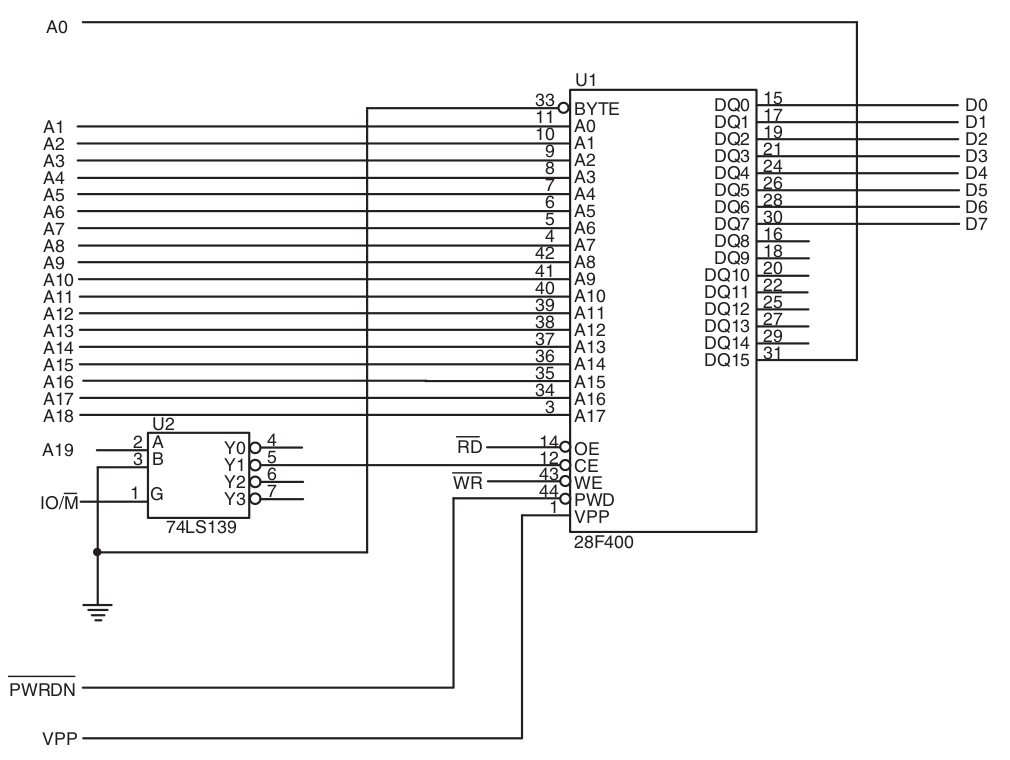
\includegraphics[width = 0.8\textwidth]{./figures/Flash_mem.png}
  \caption{The 28F400 flash memory device interfaced to the 8088 microprocessor.}
  \label{}
\end{figure}
\begin{itemize}
  \item \textbf{28F400} can be used either as a 512K x 8 or as a 512K x 16 memory device. For interfacing with 8088, it is used as a 512K x 8
  \item New pins in flash memory compared to SRAM :
  \begin{enumerate}
    \item VPP, which is connected to 12V for erasing and programming
    \item $\overline{PWD}$, which selects power down mode when a logic 0 is applied and also used for programming.
    \item BYTE, which selects byte(0) or word(1) operation.
  \end{enumerate}

  \item Pin \textbf{DQ15} functions as the least-signifcant address input when operated in byte mode
  \item Flash memory is much slower than SRAM (can need around $10^7 times$ more time).
  \item The single decoder (\textbf{74LS139}) uses address connection A19 and $IO/\overline{M}$ as inputs (location in the example : \textbf{80000H-FFFFFH})
\end{itemize}

\section{Parity for memory error detection}

\begin{figure}[h!]
  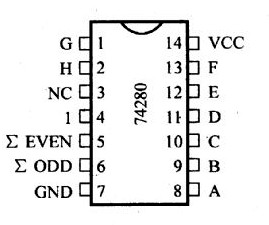
\includegraphics[width = 0.5\textwidth]{./figures/74LS280.jpeg}
  \caption{9-bit parity generator/decoder}
  \label{}
\end{figure}
\begin{table}[h!]
\centering
\begin{tabular}{ |p{6cm}|p{2cm}|p{2cm}| }
\hline
\textbf{Input}: Number of Logic 1's in A-I (9 pins)& \multicolumn{2}{|c|}{Outputs}\\

& $\sum Even$ & $\sum Odd$ \\
\hline
0,2,4,6,8   & H & L\\
1,3,5,7,9   & L & H\\
\hline
\end{tabular}

\caption{Number of chips required for fully buffered microprocessor}
\label{table:8}
\end{table}
\newpage
Example below shows 64K x 8 statis RAM using two 62556 (32K x 8) SRAMs having a parity bit stored in 6287 (64k x 1) SRAM generated by 74AS280
\newline
Decoded memory space is at \textbf{80000H-8FFFFH}.
\begin{figure}[h!]
  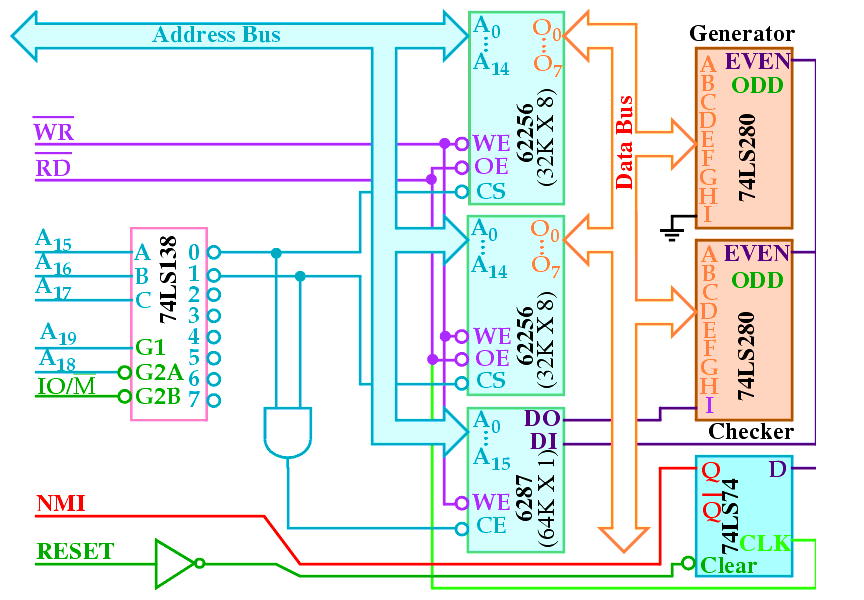
\includegraphics[width = 0.9\textwidth]{./figures/Parity.png}
  \label{fig:parity}
\end{figure}
In Figure \ref{fig:parity} as I of first \textbf{74LS280} is grounded, a 1 is stored in the parity RAM \textbf{6287}. If an even number of 1's appear in the data bus (connected to A-H). Thus, including the stored parity bit, an odd parity is stored for each byte.
\newline
\begin{itemize}
  \item \textbf{Parity SRAM}: No $\overline{OE}$ connection for $\overline{RD}$. It reads data from output pin when selected ($\overline{CE}$ is enabled) and writes data when selected with $\overline{WE} = 0$.
  \item If overall parity is odd (everything is okay), the even parity output of second \textbf{74LS280} will become logic 1. The parity output is connected to 8088's NMI.
  \item Dataread from the memory are settled to the final state before an NMI input (error detection) occurs through being timed by a D flip-flop
  \item The DFF latches output of the parity checker \textbf{74LS280} at the end of an $\overline{RD}$ cycle on the memory.
\end{itemize}

\section{Error correction}
\begin{itemize}
  \item \textbf{74LS636} : An -bit error correction and detection circuit that corrects any single bit memory read error and flags any 2-bit error.
  \item Corrects error by storing five parity bits with each byte of memory data.
  \item If more than two bits are in error(rare), the circuit ,may \textbf{not} detect it.
  \item Whenever a memory component fails completely, its bits are all high or all low. In this case, the circuit flags the processor with a multi-bit error detection.
  \item 8 data pins, 5 check bit pins, 2 control pins( S0 and S1 ), and 2 error outputs (\textbf{Single Error Flag}(SEF) and \textbf{Double Error Flag}(DEF))
\end{itemize}

\begin{table}[h!]
\centering
\begin{tabular}{ |p{1cm}|p{1cm}|p{3cm}|p{1cm}|p{1cm}| }
\hline
$S_0$ & $S_1$ & Function & SEF & DEF\\
\hline
0 & 0 & Write check word  & 0 & 0\\
\rowcolor{cyan} 0 & 1 & Correct data word & * & *\\
1 & 0 & Read data         & 0 & 0\\
1 & 1 & Latch data        & * & *\\

\hline
\end{tabular}

\caption{Control inputs for 74LS636}
\label{table:9}
\end{table}
\textbf{* : \textit{These levels are determined by the type of error}}
\begin{itemize}
  \item When a single error is detected, the \textbf{74LS636} goes through an error correction cycle: \newline
  It places 01 on S0 and S1 by causing a wait and then read following error correction.
  \item Difference in connection in memory components :\newline
  $\overline{S}$ is grounded, which enable data to be accessed from memory before $\overline{RD}$ goes low.
  \item On the next negative edge of the clock after an $\overline{RD}$, the 74LS636 checks \textbf{SEF}. If a single bit error is detected, a correction cycle causes the single-bit error to be corrected. If a double-bit error is detected, \textbf{DEF} generates an NMI.
\end{itemize}
\begin{figure}[h!]
  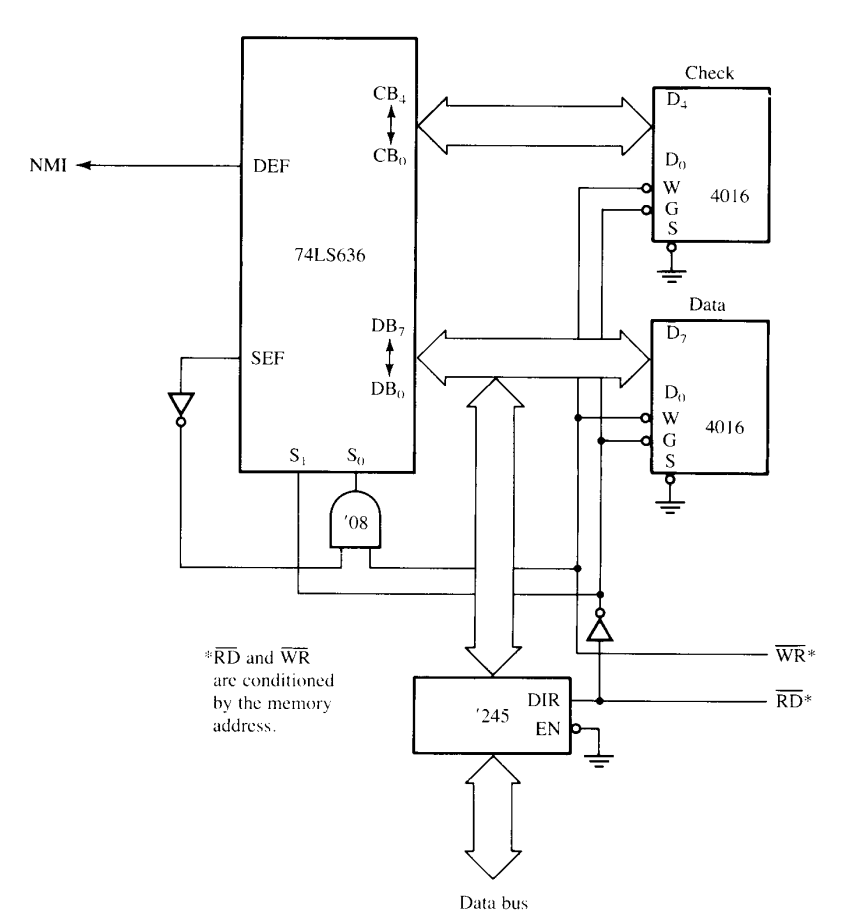
\includegraphics[width = 0.9\textwidth]{./figures/Error_Correction.png}
  \caption{An error detection and correction circuit using the 74LS636.}
  \label{}
\end{figure}
